%%%%%%%%%%%%%%%%%%%%%%%%%%%%%%%%%%%%%%%%%%%%%%%%%%%%%%%%%%%%%%%
%
% Welcome to Overleaf --- just edit your LaTeX on the left,
% and we'll compile it for you on the right. If you open the
% 'Share' menu, you can invite other users to edit at the same
% time. See www.overleaf.com/learn for more info. Enjoy!
%
%%%%%%%%%%%%%%%%%%%%%%%%%%%%%%%%%%%%%%%%%%%%%%%%%%%%%%%%%%%%%%%
\documentclass[a4paper]{article} 
 % paquets pour le français
 \usepackage{tikz}
 \usepackage{multicol}
 \usepackage[T1]{fontenc}
 \usepackage[utf8]{inputenc}
\usepackage{minted}
\definecolor{LightGray}{gray}{0.9}
  \title{Programmation C: TP1}
\author{ \textsc{Ibrahim ALAME}}
\date{6/12/2023}
\begin{document}
\maketitle

\section{Liste chaînée}
\subsection{Définition}
  %%%%%%%%%%%%%%%%%%%%%%%%%%%%%%%%%%%%%%%%%%%%%%%%%%%%%%%%%%%%%%%%%
\begin{center}
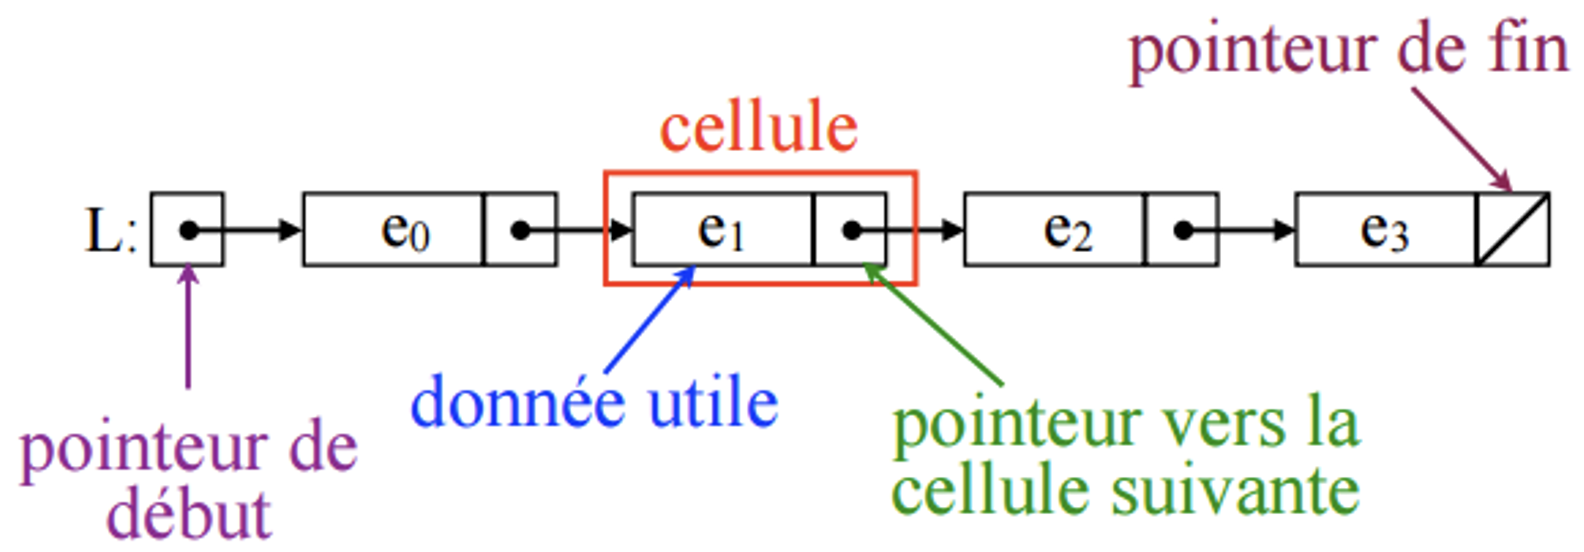
\includegraphics[scale=0.25]{liste01.png} 
\end{center}  

%%%%%%%%%%%%%%%%%%%%%%%%%%%%%%%%%%%%%%%%%%%%%%%%%%%%%%%%%%%%%%%%%
  Une liste chaînée est composée d'un ensemble d'éléments qu'on appelle ici des cellules. On veut donc, pour ce TP, construire une liste chaînée qui contient des entiers, un entier par cellule. Et qui doit en plus avoir un pointeur dans chacune de ces cellules pour créer la liaison entre elles afin de pouvoir se déplacer tout au long de la liste chaînée. Ce pointeur doit contenir l'adresse de la cellule suivante, et si on appelle la structure utilisée {\tt Element}, le type de ce pointeur sera alors {\tt struct Element}.
\begin{minted}[
%frame=lines,
framesep=2mm,
baselinestretch=1.2,
bgcolor=LightGray,
fontsize=\small,%footnotesize,
% linenos
]{c}
typedef struct Element Element;
struct Element{
    int nombre;
    Element *suivant;
};
\end{minted}

Pour une liste chaînée, il faut toujours garder dans l'esprit qu'un pointeur vers la première cellule de la liste doit être gardé quelque part, en général dans un pointeur de type struct qu'on appelle ici {\tt Liste}.

\begin{minted}[
%frame=lines,
framesep=2mm,
baselinestretch=1.2,
bgcolor=LightGray,
fontsize=\small,%footnotesize,
% linenos
]{c}
typedef struct Liste Liste;
struct Liste{
    Element *suivant;
};
\end{minted}
\subsection{Initialisation}
La fonction suivante permet d'initialiser une liste chainée:

\begin{minted}[
%frame=lines,
framesep=2mm,
baselinestretch=1.2,
bgcolor=LightGray,
fontsize=\small,%footnotesize,
% linenos
]{c}
Liste *initialisation(){
    Liste* liste = malloc(sizeof(*liste));
    Element *element = malloc(sizeof(*element));
    if(liste == NULL || element ==NULL) exit(EXIT_FAILURE);
    element->nombre =0;
    element->suivant = NULL;
    liste->premier = element;
    return liste;
}
\end{minted}



%%%%%%%%%%%%%%%%%%%%%%%%%%%%%%%%%%%%%%%%%%%%%%%%%%%%%%%%%%%%%%%%%
\subsection{Insertion}
  %%%%%%%%%%%%%%%%%%%%%%%%%%%%%%%%%%%%%%%%%%%%%%%%%%%%%%%%%%%%%%%%%
\begin{center}
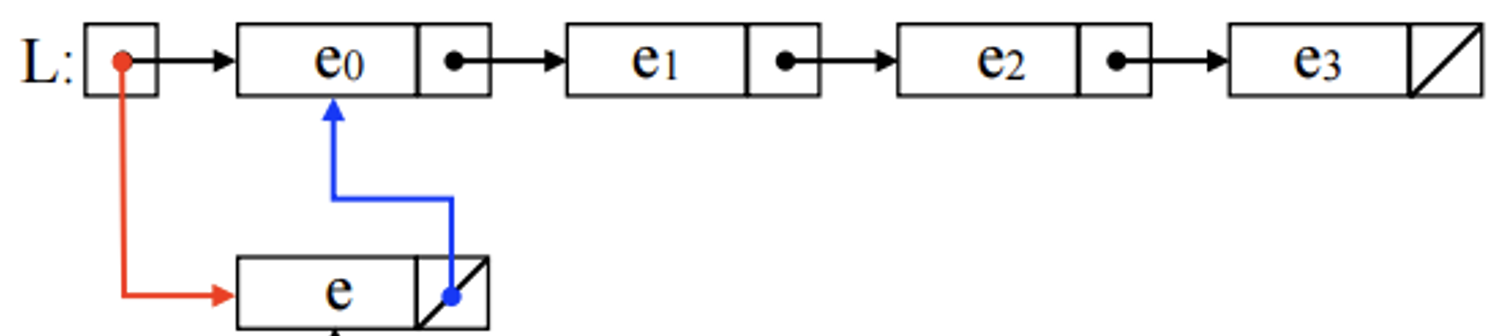
\includegraphics[scale=0.25]{liste02.png} 
\end{center}  
\begin{minted}[
%frame=lines,
framesep=2mm,
baselinestretch=1.2,
bgcolor=LightGray,
fontsize=\small,%footnotesize,
% linenos
]{c}
void insertion(Liste *liste,int nvNombre){
    /* Création du nouvel élément */
    Element *nouveau = malloc(sizeof(Element));
    if(liste == NULL || nouveau == NULL) exit(EXIT_FAILURE);
    nouveau->nombre = nvNombre;
    /* Insertion de l'élément au début de la liste */
    nouveau->suivant = liste->premier;
    liste->premier = nouveau;
}
\end{minted}

%%%%%%%%%%%%%%%%%%%%%%%%%%%%%%%%%%%%%%%%%%%%%%%%%%%%%%%%%%%%%%%%%
\subsection{Supprimer un élément}
  %%%%%%%%%%%%%%%%%%%%%%%%%%%%%%%%%%%%%%%%%%%%%%%%%%%%%%%%%%%%%%%%%
\begin{minted}[
%frame=lines,
framesep=2mm,
baselinestretch=1.2,
bgcolor=LightGray,
fontsize=\small,%footnotesize,
% linenos
]{c}
void suppression(Liste *liste){
    if(liste == NULL) exit(EXIT_FAILURE);
    if(liste->premier != NULL){
        Element *aSupprimer = liste->premier;
        liste->premier = liste->premier->suivant;
        free(aSupprimer);
    }
}
\end{minted}
%%%%%%%%%%%%%%%%%%%%%%%%%%%%%%%%%%%%%%%%%%%%%%%%%%%%%%%%%%%%%%%%%
\subsection{Afficher la liste chaînée}
  %%%%%%%%%%%%%%%%%%%%%%%%%%%%%%%%%%%%%%%%%%%%%%%%%%%%%%%%%%%%%%%%%
\begin{minted}[
%frame=lines,
framesep=2mm,
baselinestretch=1.2,
bgcolor=LightGray,
fontsize=\small,%footnotesize,
% linenos
]{c}
void afficherListe(Liste *liste){
    if(liste == NULL) exit(EXIT_FAILURE);
    Element *actuel = liste->premier;
    while (actuel != NULL){
        printf("%d -> ",actuel->nombre);
        actuel = actuel->suivant;
    }
    printf("NULL\n");
}
\end{minted}
%%%%%%%%%%%%%%%%%%%%%%%%%%%%%%%%%%%%%%%%%%%%%%%%%%%%%%%%%%%%%%%%%
\subsection{Exemple}
  %%%%%%%%%%%%%%%%%%%%%%%%%%%%%%%%%%%%%%%%%%%%%%%%%%%%%%%%%%%%%%%%%
\begin{minted}[
%frame=lines,
framesep=2mm,
baselinestretch=1.2,
bgcolor=LightGray,
fontsize=\small,%footnotesize,
% linenos
]{c}
int main(){
    Liste* L = initialisation();
    insertion(L,4);
    insertion(L,8);
    insertion(L,15);
    afficherListe(L);
    suppression(L);
    afficherListe(L);
    
    return 0;
}
\end{minted}
\section{Représentation d'une matrice creuse}
On définit une matrice creuse comme étant une matrice dont plus que la moitié des éléments sont nuls.
\[\left(\begin{array}{cccccc}
0 & 7 & 0 & 5 & 0 & 0 \\
6 & 0 & 0 & 0 & 0 & 5 \\
0 & 0 & 1 & 0 & 0 & 0 \\
0 & 0 & 0 & 0 & 0 & 0 
\end{array}\right)\]
Pour minimiser l'espace occupé par ce type de matrice on choisi de la représenter sous forme d'un tableau de listes chaînées, de sorte que la i$^{\tiny\mbox{ième}}$ liste chaînée contient les éléments non nuls de la ligne i de la matrice et chacun d'eux accompagné du numéro de la colonne où il se trouve.
\begin{center}
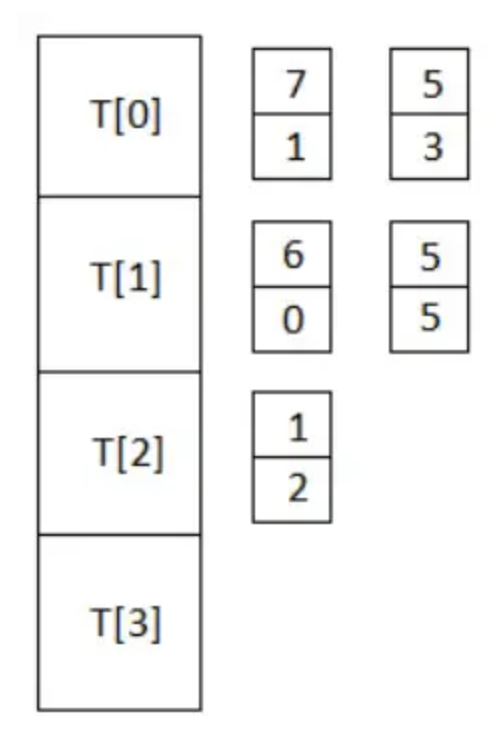
\includegraphics[scale=0.25]{liste03.png} 
\end{center}  
Tâches à faire:
\begin{enumerate}
\item Définir la structure qui sera utilisée pour les cellules des listes chaînées;
\item Transformer une matrice $M$ de taille $n\times m$ en tableau de listes chaînées $T$ comme défini précédemment;
\item Afficher un élément $M_{i,j}$ à partir de $T$.
\end{enumerate}
\section{Manipulation d'une liste chaînée}
\begin{enumerate}
\item Écrire un programme C qui crée et lit une liste chaînée d'entiers, et lit ensuite un entier et une position et insère l'entier dans la position précisée.
\item Écrire un programme C qui crée et lit une liste chaînée d'entiers, puis supprime de cette liste toutes les occurrences d'un entier entré par l'utilisateur.
\item Écrire un programme C qui inverse une liste chaînée en manipulant seulement ses pointeurs de liaison.
\end{enumerate}
\end{document}
